\section{Spontaneous emission}
The initial state of the system in the figure is:
\begin{align}
    \ket{\psi}=\ket{e}\otimes\ket{\{0\}},\quad\ket{\{0\}}=\text{All field modes in vacuum state}.
\end{align}
\begin{figure}[htbp]
    \centering
    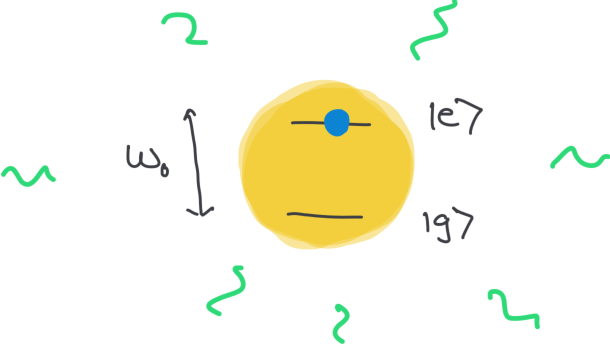
\includegraphics[width=.25\columnwidth]{PartOne/ChapterFour/figures/spontaneousemission_initialstate.png}
    \caption{Initial state}
\end{figure}

We observe that the total Hamilonian in the SP
\begin{align*}
    H_{tot}=\hbar\omega_0\hsigma_+\hsigma_-+\sum_{\bk,\lambda}\hbar\omega_{\bk}\ha^\dagger_{\bk,\lambda}\ha_{\bk,\lambda}+
    \hbar\sum_{\bk,\lambda}(g_{\bk,\lambda}\hsigma_+\ha_{\bk,\lambda}+g_{\bk,\lambda}^*\hsigma_-\ha^\dagger_{\bk,\lambda}).
\end{align*}
preserves the total number of exctiations in atom + field supbspaces
\begin{align*}
    \hN_{AF}&=\hsigma_+\hsigma_-+\sum_{\bk,\lambda}\ha^\dagger_{\bk,\lambda}\ha_{\bk,\lambda}\\
    [\hN_{AF},\hH_{tot}]=0&\Longrightarrow\shortstack{Total number of atoms+field exctiations is\\preserved by the dynamics under $H_{tot}$}
\end{align*}
We can thus maeke the following onsate for th eatom+field stat at any time $t$:
\begin{align}
    \ket{\psi(t)}=c_e(t)\ket{\{0\}}+\sum_{\bk,\lambda}c_{g,\bk,\lambda}(t)\ket{g}\ket{1_{\bk,\lambda}}
\end{align}
Let us qrite the dynamics of the quantum state in the interaction picture:
\begin{align*}
    i\hbar\partial_t\ket{\psi(t)}=&\tilde{H}_{int}\ket{\psi(t)}\\
    i\hbar\partial_t[c_e(t)\ket{\{0\}}+\sum_{\bk,\lambda}c_{g,\bk,\lambda}(t)\ket{g}\ket{1_{\bk,\lambda}}]=&\left[\sum_{\bk,\lambda}g_{\bk,\lambda}\hsigma_+
    \ha_{\bk,\lambda}e^{-i(\omega_{\bk}-\omega_0)t}+g_{\bk,\lambda}^*\hsigma_-\ha^\dagger_{\bk,\lambda}e^{i(\omega_{\bk}-\omega_0)t}\right]\\
    &\times\left[
        c_e(t)\ket{e}\ket{\{0\}}+\sum_{\bk',\lambda'}c_{g,\bk',\lambda'}(t)\ket{g}\ket{1_{\bk',\lambda'}}\right]\\
        i\hbar\partial_tc_e\ket{e}\ket{\{0\}}+i\hbar\sum_{\bk,\lambda}\partial_tc_{g,\bk,\lambda}\ket{g}\ket{1_{\bk,\lambda}}&\stackrel{(a)}{=}\hbar\sum_{\bk,\lambda}
        \left(g_{\bk,\lambda}c_{g,\bk,\lambda}e^{-i(\omega_{\bk}-\omega_0)t}\ket{e}\ket{\{0\}}+g^*_{\bk,\lambda}
        c_ee^{i(\omega_{\bk}-\omega_0)t}\ket{g}\ket{1_{\bk,\lambda}}\right)
\end{align*}
In $(a)$, we used the fact that $\ha_{\bk,\lambda}\ket{1_{\bk',\lambda'}}=\delta^3(\bk-\bk')\delta_{\lambda\lambda'}$. Comparing coefficients for 
$\ket{e}\ket{\{0\}}$ and $\ket{g}\ket{1_{\bk,\lambda}}$:
\begin{align*}
    i\partial_tc_e&=\sum_{\bk,\lambda}g_{\bk,\lambda}c_{g,\bk,\lambda}e^{-i(\omega_{\bk}-\omega_0)t}\\
    i\partial_tc_{g,\bk,\lambda}&=g^*_{\bk,\lambda}c_ee^{i(\omega_{\bk}-\omega_0)t}
\end{align*}
We are interested in $c_e(t)$, so we will eliminate $c_{g,\bk,\lambda}(t)$ from the equation of motion for the atom:
\begin{align}
    i[c_{g,\bk,\lambda}(t)-\cancelto{0}{c_{g,\bk,\lambda}(0)}]=g^*_{\bk,\lambda}\int_0^td\tau\;c_e(\tau)e^{i(\omega_{\bk}-\omega_0)\tau},
\end{align}
where $c_{g,\bk,\lambda}(0)=0$ as there are no excitation in the field in the beginning. Substituting this coeficient in the equation of motion of the 
atom:
\begin{align*}
    i\partial_tc_e&=-i\sum_{\bk,\lambda}|g_{\bk,\lambda}|^2\int_0^td\tau\;c_e(\tau)e^{-i(\omega_{\bk}-\omega_0)(t-\tau)}\\
    \partial_tc_e&=-\sum_{\bk,\lambda}|g_{\bk,\lambda}|^2\int_0^td\tau'\;e^{-i(\omega_{\bk}-\omega_0)\tau'}c_e(t-\tau')\quad(\tau'=t-\tau)
\end{align*}
At this point we make the \emph{Markov approximation} which means that the system evolution at any time is determine by its present state $c_e(t)$.
Thus, aproximating $c_e(t-\tau')\to c_e(t)$ in the integral, we obtain:
\begin{align*}
    \partial_tc_e\approx-c_e(t)\sum_{\bk,\lambda}|g_{\bk,\lambda}|^2\int_0^td\tau\;e^{-i(\omega_{\bk}-\omega_0)(t-\tau)}=-\frac{\gamma_0}{2}c_e(t). 
\end{align*}
And finally,
\begin{align}
    c_e(t)=e^{-\gamma_0t/2}c_e(0)\Longrightarrow |c_e(t)|^2=e^{-\gamma_0},
\end{align}
which is an exponential decay of an excited atom probability at a rate $\gamma_0$.

